\documentclass[11pt]{article}
\usepackage[margin=1.05in,headheight=14pt]{geometry}
\usepackage[T1]{fontenc}
\usepackage{lmodern,microtype,amsmath,amssymb,amsthm,booktabs,tikz}
\usepackage{xcolor}
\definecolor{linknavy}{RGB}{25,55,125}
\usepackage[colorlinks=true,linkcolor=linknavy,citecolor=linknavy,urlcolor=linknavy]{hyperref}
\usepackage{orcidlink,fancyhdr}
\newtheorem{theorem}{Theorem}
\newtheorem{corollary}[theorem]{Corollary}
\newtheorem{lemma}[theorem]{Lemma}
\theoremstyle{remark}
\newtheorem{remark}[theorem]{Remark}
\newcommand{\dd}{\mathrm{d}}
\newcommand{\e}{\mathrm{e}}

% Page-1 header block (conventions/manuscript-header-standard.md). The four document
% macros are set by the publishing tool when the version DOI is reserved. At this text
% width the two DOIs do not fit on one line of the box, so each has its own line.
\newcommand{\doctype}{Preprint}
\newcommand{\docversion}{v0.04}
\newcommand{\docdate}{18 September 2026}
\newcommand{\versiondoi}{10.5281/zenodo.22835072}
\newcommand{\conceptdoi}{10.5281/zenodo.22315251}
\newcommand{\docrepo}{github.com/fsantibanezleal/CAOS\_RESEARCH}
\newcommand{\headerblock}{%
\begin{center}
\fbox{\parbox{0.94\textwidth}{\small\raggedright
\textbf{\doctype} \quad$\cdot$\quad \docversion, \docdate \quad$\cdot$\quad Licence CC BY 4.0\\[2pt]
CAOS Research open-problems programme \quad$\cdot$\quad problem \texttt{bougard-joret}\\[2pt]
Version DOI \href{https://doi.org/\versiondoi}{\texttt{\versiondoi}}\\[2pt]
Concept DOI (always latest) \href{https://doi.org/\conceptdoi}{\texttt{\conceptdoi}}\\[2pt]
Not peer reviewed. Source code, data and computational records: \href{https://\docrepo}{\texttt{\docrepo}}
}}
\end{center}
\vspace{4pt}}

\pagestyle{fancy}
\fancyhf{}
\fancyhead[L]{\small CAOS Research \doctype}
\fancyhead[R]{\small First interior shell\textperiodcentered\ \docversion}
\fancyfoot[C]{\thepage}
\fancypagestyle{plain}{\fancyhf{}\fancyfoot[C]{\thepage}\renewcommand{\headrulewidth}{0pt}}
\title{The first interior shell of the\\Bougard--Joret extremal problem}
\author{Felipe Santib\'a\~nez-Leal\,\orcidlink{0000-0002-0150-3246}\\
\small CAOS Research program\\
\small\texttt{github.com/fsantibanezleal/CAOS\_RESEARCH}}
\date{\docdate}
\begin{document}
\maketitle
\headerblock
\begin{abstract}
Let $f(n,\alpha,k)$ be the minimum size of a $k$-connected graph of order $n$ and independence number $\alpha$.
Das and Gupta recently determined the boundary $n=\alpha+k$ and disproved the proposed Bougard--Joret formula there.
We determine the entire admissible first interior shell:
$f(\alpha+k+1,\alpha,k)=\lceil k(\alpha+k+1)/2\rceil$ for every $k\ge3$ and $2\le\alpha\le k+1$.
The construction augments classical Harary graphs with complement matchings and attaches an independent set through distinct missing-neighbor pairs.
An elementary cyclic-gap proof controls connectivity, including all parity cases.
We characterize all extremizers when $\alpha=2$ as complements of unions of cycles of lengths at least five, and give the complete nonstar-tree characterization when $\alpha=k-1$.
The full-shell result is supported by 75 exact finite constructions, an independent re-implementation of the checks, and negative controls.
The universal statement follows from the proof, not from finite computation. The general revised first regime and second regime remain unresolved.
\end{abstract}

\section{Problem, prior work and scope}

All graphs are finite, simple and undirected. Write $\e(G)$ for the number of edges, $\alpha(G)$ for the maximum size of an independent set, and $\kappa(G)$ for vertex connectivity.
A graph is $k$-connected if it has more than $k$ vertices and deletion of fewer than $k$ vertices leaves it connected.

Bougard and Joret conjectured, under $n\ge2\alpha$, $n\ge\alpha+k$, $\alpha\ge2$, $k\ge3$, that
\[
f(n,\alpha,k)=
\begin{cases}
\lceil nk/2\rceil,&n\le k\alpha,\\
t(n,\alpha)+\lceil k\alpha/2\rceil,&n>k\alpha,
\end{cases}
\]
where $t(n,\alpha)$ denotes the edge count of the balanced union of $\alpha$ cliques \cite{BJ}.
Das and Gupta determine the whole boundary $n=\alpha+k$; in particular, for $k\ge4$ they prove
\begin{equation}\label{eq:old}
f(2k-1,k-1,k)=k^2-1,
\end{equation}
with extremals exactly the joins of an independent $(k-1)$-set and a tree on $k$ vertices \cite{DG}.
The original disproof and this preceding-boundary characterization are their results.

We prove the adjacent diagonal $(n,\alpha,k)=(2k,k-1,k)$ and characterize its extremizers (Theorem~\ref{thm:main}).
We extend the numerical result to every admissible parameter on $n=\alpha+k+1$ (Theorem~\ref{thm:shell}), and add a complete equality classification for $\alpha=2$ (Theorem~\ref{thm:cycles}).
The full-shell formula includes classical overlaps: $\alpha=k+1$ is covered by $n=2\alpha$ in \cite{BJ}, and $(n,\alpha,k)=(6,2,3)$ is covered by $n=k\alpha$.
Targeted searches and the final sections of both primary problem papers revealed no formula for the entire next shell, but this is not an assertion of exhaustive bibliographic priority.
Harary's connectivity constructions \cite{Harary} are classical ingredients, not new claims of this work.

Our universal deductions are labeled [D], exact finite computations [MV], and suggested extensions [C].
The proofs and verification are recorded in EXP-001 and EXP-002 \cite{Record,ShellRecord}.

\section{The entire first interior shell}

Write $a$ for the prescribed independence number. Our main extension is the following.

\begin{theorem}[First interior shell, D]\label{thm:shell}
For every integer $k\ge3$ and every integer $2\le a\le k+1$,
\[
f(a+k+1,a,k)=\left\lceil\frac{k(a+k+1)}2\right\rceil.
\]
\end{theorem}

The restriction $a\le k+1$ is exactly $n\ge2a$ on this shell.
Also $n\le ka$, because $a(k-1)\ge k+1$ for $a\ge2$, $k\ge3$.
Every $k$-connected graph has minimum degree at least $k$, so the claimed value is a lower bound by the degree sum.
We give constructions attaining it with exact independence number $a$.

\subsection{Two elementary residual-graph lemmas}

\begin{lemma}[Matching bound]\label{lem:matching}
A nonempty graph of minimum degree at least $b\ge0$ has a matching of size at least $\lceil b/2\rceil$.
\end{lemma}
\begin{proof}
Take a maximal matching $Q$. If a vertex $v$ is unmatched, all its neighbors are matched endpoints, so $2|Q|\ge\dd(v)\ge b$.
If every vertex is matched, $2|Q|$ is the order of the graph and is at least $b+1$.
A subset of $Q$ realizes any smaller prescribed size.
\end{proof}

Number a cycle of order $m$ cyclically by $0,\ldots,m-1$.
Its $r$th power $C_m^r$ joins pairs at cyclic distance at most $r$.
We use $r\ge1$ and $m\ge2r+4$.
The following are classical Harary constructions \cite{Harary}; we include the needed connectivity proof.

\begin{lemma}[Cyclic gaps]\label{lem:harary}
The graph $C_m^r$ is $2r$-connected and $2r$-regular. The following augmentations are $(2r+1)$-connected:
\begin{enumerate}
\item For $m=2q$, add the antipodal matching $\{i,i+q\}$, $0\le i<q$.
The result is $(2r+1)$-regular.
\item For $m=2q+1$, add $\{i,i+q\}$, $0\le i\le q$.
The result has degree $2r+2$ at $q$ and degree $2r+1$ elsewhere.
\end{enumerate}
\end{lemma}
\begin{proof}
In the cyclic list of surviving vertices, consecutive survivors are adjacent if their intervening gap has fewer than $r$ deleted vertices.
With at most one larger gap, these edges form a spanning path or cycle.
Disconnection therefore requires two gaps, each with at least $r$ deletions, proving $2r$-connectivity of the cycle power.
Its degree gives the matching upper bound on connectivity.

For either odd-degree augmentation, only exactly $2r$ deletions require attention.
If the cycle power disconnects, these deletions must form exactly two blocks of length $r$, leaving two nonempty surviving arcs.
Let the shorter arc have length $p$. Rotate coordinates for the geometric argument so that
\[
A=\{0,\ldots,p-1\},\qquad B=\{p+r,\ldots,m-r-1\}.
\]
For $m=2q$, we have $p\le q-r$, and for every $x\in A$,
\[
p+r\le q\le x+q\le q+p-1\le2q-r-1.
\]
Its antipode therefore lies in $B$, yielding a surviving added edge.
For $m=2q+1$, again $p\le q-r$; both $x+q$ and $x+q+1$ lie in $B$, since their indices range from $q$ to $q+p\le2q-r$.
Every vertex in the odd-order construction has an added neighbor at one of these two almost-antipodal positions.
This property survives coordinate rotation even though the chosen edge cover need not be rotation invariant.
Thus an added edge joins the two internally connected arcs in either parity.
The endpoint lists in the odd-order construction overlap only at $q$, giving its degree pattern; the even-order added edges are a perfect matching.
\end{proof}

We will also use
\begin{equation}\label{eq:cycle-alpha}
\alpha(C_m^r)\le\left\lfloor\frac{m}{r+1}\right\rfloor.
\end{equation}
Indeed, the forward cyclic distances between consecutive members of an independent set of size at least two are all at least $r+1$, and sum to $m$.
A singleton also satisfies the bound.

\subsection{An injective missing-neighbor lemma}

\begin{lemma}[Residual lift]\label{lem:lift}
Let $k\ge a\ge3$, $d=k-a$, and let $H$ have order $k+1$.
Choose $M\subseteq V(H)$ with $|M|=a$. Suppose that $\alpha(H)\le a$, that
\[
\dd_H(t)\ge
\begin{cases}d+1,&t\in M,\\d,&t\notin M,\end{cases}
\]
and, when $d\ge1$, that $H$ is $d$-connected.
Add an independent set $S$ of size $a$, put it in bijection with $M$, and join each $s\in S$ to every vertex of $H$ except its assigned vertex.
Then the resulting graph $G$ has $\alpha(G)=a$ and $\kappa(G)=k$.
\end{lemma}
\begin{proof}
Each vertex of $S$ has degree $k$.
With $r_t=1$ for $t\in M$ and $r_t=0$ otherwise,
\[
\dd_G(t)=\dd_H(t)+a-r_t\ge k.
\]
An independent set within either part has size at most $a$.
A mixed independent set contains at most one residual vertex, since a vertex of $S$ misses only one vertex of $H$.
It contains at most one vertex of $S$, since the misses are distinct.
Its size is therefore at most two. The set $S$ witnesses equality $\alpha(G)=a$.

Delete $X$ with $|X|<k$, and write $A=S\setminus X$, $B=V(H)\setminus X$.
Always $|B|\ge2$.
If $A$ is empty, $d=0$ is impossible and fewer than $d=k-a$ residual vertices were deleted, so $d$-connectivity of $H$ suffices.

Suppose $A\ne\varnothing$ and $|B|\ge3$.
Any two vertices of $A$ share a neighbor in $B$, so all of $A$ and every member of $B$ adjacent to it lie in a common component $C$.
At most one residual vertex $t$ can lie outside $C$; it is missed by all of $A$, so $|A|\le r_t$.
If it is disconnected, all its $H$-neighbors have been deleted. Hence
\[
|X|\ge a-|A|+\dd_H(t)\ge a-r_t+\dd_H(t)=\dd_G(t)\ge k,
\]
a contradiction.

If $|B|=2$, precisely $k-1$ residual vertices were deleted, and all of $S$ survives.
Since its $a\ge3$ vertices miss distinct residual vertices, some $s\in S$ is adjacent to both members of $B$.
Every other member of $S$ is adjacent to at least one of them, so the remainder is connected.
Thus $\kappa(G)\ge k$, while the degree-$k$ vertices in $S$ give equality.
\end{proof}

\subsection{The generic residual construction}

Set $m=k+1=a+d+1$, $n=a+m$, $\varepsilon=kn\bmod2$, and $r=\lfloor d/2\rfloor\ge1$.
We construct a $d$-connected residual graph $H$ with degree $d+1$ at exactly $a+\varepsilon$ distinct vertices and degree $d$ elsewhere.
Every case contains $C_m^r$.

If $d=2r$, start with $C_m^r$.
Its complement is $a$-regular, and $\varepsilon$ is the parity of $a$ because $n=2a+d+1$ is odd.
Lemma~\ref{lem:matching} supplies a complement matching of size $(a+\varepsilon)/2$.
Adding it raises exactly $a+\varepsilon$ degrees by one.

If $d=2r+1$ and $m$ is even, start with the antipodal augmentation in Lemma~\ref{lem:harary}.
It is $d$-regular, its complement is $a$-regular, $a$ is even, and $\varepsilon=0$.
Add a complement matching of size $a/2$.

If $d=2r+1$ and $m=2q+1$ is odd, start with the odd-order augmentation.
Its unique higher-degree vertex is $w=q$.
Here $a$ is odd and $\varepsilon=0$.
Every other vertex has degree $a$ in the complement; after deleting $w$, that complement has minimum degree at least $a-1$.
Add a matching of size $(a-1)/2$ in it.
Its endpoints avoid $w$, so precisely $a$ vertices now have degree $d+1$.
All three constructions preserve the starting graph's $d$-connectivity.

By \eqref{eq:cycle-alpha} and $d\le2r+1$,
\[
m=a+d+1\le a+2r+2<(a+1)(r+1),\qquad \alpha(H)\le a.
\]
The strict inequality follows from $r(a-1)-1\ge1$.
Choose any $a$ higher-degree vertices for $M$ and apply Lemma~\ref{lem:lift}.
Every vertex in $S$ and every selected residual vertex has degree $k$.
The residual vertices of degree $d$ also have total degree $k$.
When $\varepsilon=1$, the sole unselected higher-degree vertex has total degree $k+1$.
Consequently
\[
\e(G)=\frac{kn+\varepsilon}{2}=\left\lceil\frac{kn}{2}\right\rceil,
\]
proving Theorem~\ref{thm:shell} in this range.

\subsection{The remaining parameters}

For $a=k$, take a residual matching of $\lceil k/2\rceil$ edges on $k+1$ vertices and choose $k$ distinct endpoints for $M$.
Its independence number is $k+1-\lceil k/2\rceil\le k$.
Lemma~\ref{lem:lift} applies with $d=0$, without requiring residual connectivity.
For even $k$, all degrees in $G$ are $k$; for odd $k$, the single unselected matching endpoint has total degree $k+1$ and every other degree is $k$.
Thus the required edge bound is attained.

For $a=k-1$ and $k\ge4$, use $H=P_{k+1}$ and let $M$ be its $k-1$ internal vertices.
The path is connected, its selected degrees are two, its remaining degrees are one, and
\[
\alpha(P_{k+1})=\left\lceil\frac{k+1}{2}\right\rceil\le k-1.
\]
Lemma~\ref{lem:lift} with $d=1$ gives a $k$-regular extremal graph.
The stronger complete tree characterization from version 0.01 is retained in Theorem~\ref{thm:main} below.
Its $k=3$ case is covered by $a=2$.

For $a=k+1$, use the crown graph $K_{a,a}$ minus a perfect matching.
It is $k$-regular, and its independence number is $a$: a mixed independent set has size at most two, while each part has size $a$.
After fewer than $a-1$ deletions, at least two vertices survive in each part and at least $a+2\ge6$ survive in total.
One part therefore has at least three vertices.
Any two vertices in the other part share a neighbor there, and every remaining vertex has a neighbor across the bipartition.
The surviving graph is connected.

The last case, $a=2$, gives an additional equality classification.

\begin{theorem}[Cycle-complement extremizers, D]\label{thm:cycles}
For $k\ge3$ and $n=k+3$, all extremizers for $f(n,2,k)$ are precisely the complements of disjoint unions of cycles of lengths at least five, with total order $n$.
\end{theorem}
\begin{proof}
Let $F$ be such a cycle union and $G=\overline F$.
Then $G$ is $(n-3)$-regular and $\alpha(G)=\omega(F)=2$.
The degree sum $n(n-3)$ is even, giving $\e(G)=nk/2$.
If fewer than $k=n-3$ deletions disconnected $G$, at least four vertices would survive.
Partition the surviving components into nonempty sets $U,V$ with no $G$-edges between them.
All cross pairs belong to $F$.
Since $F$ has maximum degree two, $|U|,|V|\le2$, so both must equal two.
Their four cross edges consume all endpoint degrees and form a whole $4$-cycle component of $F$, a contradiction.
Taking $F=C_n$ provides an example for every $n\ge6$, completing the numerical proof of Theorem~\ref{thm:shell}.

Conversely, equality and minimum degree at least $k$ force an extremizer to be $k$-regular, so its complement is $2$-regular.
It is therefore a union of cycles.
Triangles violate $\alpha(G)=2$.
For a $4$-cycle component, delete all $n-4=k-1$ vertices outside it; its complement consists of two disjoint edges, contradicting $k$-connectivity.
Every cycle must have length at least five, and the first part proves sufficiency.
\end{proof}

The constructions exhaust $2\le a\le k+1$: either $a=2$, $a\in\{k-1,k,k+1\}$, or $a\ge3$ and $k-a\ge2$.
Only the cycle-complement and tree-strip subfamilies receive complete equality classifications here.


\section{The tree construction and the extremal theorem}

For a tree $T$ on $k+1$ vertices, let $S$ be a disjoint independent set of size $k-1$.
Partition $S$ into fibers $(S_t:t\in V(T))$ satisfying
\begin{equation}\label{eq:fiber}
|S_t|=\dd_T(t)-1.
\end{equation}
Keep all edges of $T$, and for each $s\in S_t$ add edges from $s$ to every tree vertex except $t$.
Call the resulting graph $G(T,(S_t))$.
The required partition exists because
\begin{equation}\label{eq:sum}
\sum_{t\in V(T)}(\dd_T(t)-1)=2k-(k+1)=k-1.
\end{equation}

\begin{theorem}[Adjacent exceptional strip, D]\label{thm:main}
For every integer $k\ge3$,
\[
f(2k,k-1,k)=k^2.
\]
A graph is extremal for these parameters if and only if it is isomorphic to $G(T,(S_t))$ for a nonstar tree $T$ on $k+1$ vertices and fibers satisfying \eqref{eq:fiber}.
Every extremal graph has this representation relative to each of its maximum independent sets.
\end{theorem}

\begin{figure}[ht]
\centering
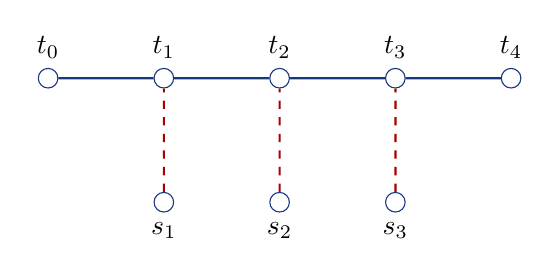
\begin{tikzpicture}[scale=1.05,vertex/.style={circle,draw=linknavy,fill=white,inner sep=2.5pt}]
\foreach \i in {0,...,4}{\node[vertex,label=above:{$t_{\i}$}] (t\i) at (1.4*\i,1.5) {};}
\foreach \i in {0,...,3}{\pgfmathtruncatemacro{\j}{\i+1}\draw[thick,linknavy] (t\i)--(t\j);}
\foreach \i in {1,...,3}{\node[vertex,label=below:{$s_{\i}$}] (s\i) at (1.4*\i,0) {};
\draw[dashed,red!65!black,thick] (s\i)--(t\i);}
\end{tikzpicture}
\caption{The $k=4$ path construction. The solid path is $T=P_5$; the three dashed pairs are \emph{nonedges}. Add every other pair between the two rows, and no pair within the lower row. This yields an eight-vertex, 16-edge extremal graph.}
\label{fig:path}
\end{figure}

\subsection{Regularity and independence}

Every vertex of $S$ has degree $k$. At a tree vertex $t$,
\[
\dd_G(t)=\dd_T(t)+(k-1)-|S_t|=k.
\]
Thus the graph is $k$-regular, has order $2k$, and has $k^2$ edges.

A nonstar tree of order $k+1$ cannot contain an independent $k$-set: all its edges would then meet the remaining vertex, and connectedness would force a star.
Consequently $\alpha(T)\le k-1$, and also $\dd_T(t)\le k-1$ for every $t$.
An independent set contained in either $S$ or $T$ therefore has size at most $k-1$.
An independent set meeting both parts contains only one tree vertex $t$, because each member of $S$ has only one nonneighbor in $T$.
Its other vertices lie in $S_t$, so its size is at most
\[
1+|S_t|=\dd_T(t)\le k-1.
\]
Since $S$ is itself independent, $\alpha(G)=k-1$.

\subsection{Connectivity}

Let $X\subseteq V(G)$ satisfy $|X|<k$, and set
\[
A=S\setminus X,\qquad B=V(T)\setminus X.
\]
There are at least two vertices in $B$.
If $A$ is empty, deletion of all $k-1$ vertices of $S$ uses the available deletion budget. Hence $G-X=T$ is connected.

Assume $A\ne\varnothing$ and $|B|\ge3$.
Any two vertices of $A$ share a neighbor in $B$, since each misses at most one member of $B$.
All of $A$, and all tree vertices adjacent to at least one member of $A$, therefore lie in a common component $C$.
At most one tree vertex $t$ can remain outside $C$: such a vertex must be the unique missed vertex of every member of $A$, so $A\subseteq S_t$.
If $t$ is disconnected from $C$, all its tree neighbors must have been deleted.
All vertices of $S\setminus A$ were also deleted, and these sets are disjoint. Therefore
\begin{align*}
|X|&\ge k-1-|A|+\dd_T(t)\\
&\ge k-1-|S_t|+\dd_T(t)=k,
\end{align*}
a contradiction.

The case $|B|=2$ requires a different argument.
Write $B=\{u,v\}$. Exactly $k-1$ tree vertices have been deleted, so every member of $S$ survives.
If a vertex of $S$ misses a tree vertex other than $u,v$, it is adjacent to both $u$ and $v$.
Every other member of $S$ is adjacent to at least one of them, proving connectedness.
Otherwise the only nonempty fibers are $S_u,S_v$.
By \eqref{eq:fiber}, every other tree vertex is a leaf.
Since $T$ is nonstar, $u,v$ are exactly its two nonleaf vertices, and they must be adjacent: an internal vertex on their path would be a third nonleaf vertex.
The surviving edge $uv$ reconnects the graph.
Thus $G$ is $k$-connected in every case.

\subsection{Optimality and all equality cases}

Any $k$-connected graph on $2k$ vertices has minimum degree at least $k$ and hence at least $k^2$ edges.
The constructed graphs attain this lower bound, proving the numerical statement.

Conversely, let $G$ be extremal, and let $S$ be any maximum independent set, of order $k-1$.
Equality in the degree-sum lower bound forces $k$-regularity.
The residual graph $H=G-S$ has $k+1$ vertices and is connected, since fewer than $k$ vertices were deleted.
Each vertex of $S$ misses exactly one vertex of $H$.
There are $k(k-1)$ edges between $S$ and $H$, leaving
\[
\e(H)=k^2-k(k-1)=k.
\]
Thus $H$ is a tree.
Writing $S_t$ for the vertices that miss $t$, regularity gives
\[
k=\dd_H(t)+(k-1)-|S_t|,
\]
so \eqref{eq:fiber} holds.
If $H$ were a star, its $k$ leaves would form an independent set in $G$, contrary to $\alpha(G)=k-1$.
This completes the proof of Theorem~\ref{thm:main}.\hfill$\square$

\begin{remark}
The theorem characterizes graphs relative to a marked maximum independent set.
It does not assert a bijection between nonstar trees and unmarked graph isomorphism classes.
Different maximum independent sets in the same graph need not give a uniquely determined representation without a further argument.
\end{remark}

\section{Boundary transition and a residual-graph viewpoint}

Combining Theorem~\ref{thm:main} with \eqref{eq:old} gives the following precise transition.
\begin{corollary}[D, using the preceding-boundary theorem of \cite{DG}]
For every $k\ge4$,
\[
f(2k,k-1,k)-f(2k-1,k-1,k)=1.
\]
The excess over the degree-sum prediction drops from $\lfloor k/2\rfloor-1$ to zero.
\end{corollary}
\begin{proof}
The values are $k^2$ and $k^2-1$.
At order $2k-1$, the prediction is $\lceil k(2k-1)/2\rceil=k^2-\lfloor k/2\rfloor$; at order $2k$ it is $k^2$.
\end{proof}

The mechanism differs from simply adding a vertex to a preceding-boundary extremal graph.
On the original boundary every independent-set vertex is adjacent to every residual vertex.
On the new diagonal it misses exactly one. The sizes of these missing-neighbor fibers compensate for the residual tree degrees, making every total degree equal to $k$.
Connectivity must still be proved separately; the double-star case shows why a common-neighbor argument alone is insufficient.

\section{Exact validation and negative controls}

The computations \cite{Record,ShellRecord} are finite.
They support the proof by testing constructions and implementation failure modes; they are not the source of the universal quantifier.
All arithmetic is integer and all choices are deterministic.

\subsection{Full-shell controls, EXP-002}

The full grid contains every $k=3,\ldots,12$ and every $a=2,\ldots,k+1$, totaling 75 graphs.
All pass exact degree and edge counts, recursive independence, and vertex-split max-flow connectivity.
For the 45 graphs of order at most 16, direct subset enumeration and exhaustive vertex deletion agree with those checks.
The 36 Harary cases also pass both connectivity checks on their starting and augmented residual graphs.
The 15 odd-degree-sum cases each have exactly one degree-$(k+1)$ vertex.
Deleting an edge incident to a degree-$k$ vertex is rejected in every one of the 75 constructions.
Eight complement-cycle controls test triangles, $4$-cycles, and unions of longer cycles.
A regenerated census of all 32,768 labeled order-six graphs finds 60 extremizers, exactly the complements of six-cycles.
This census shares the checker library of EXP-001; it is an independent regeneration, not a wholly independent implementation.

A separate implementation using NetworkX 3.4.1 reconstructs the saved raw edge lists without importing either CAOS graph checker.
Exact node connectivity and maximal cliques of the complement independently verify connectivity and independence for all 75 graphs.
It also verifies the 36 residual constructions, all damaged-edge controls, and the cycle controls.
Its output file records the SHA-256 digests of the proof, the certificate and the verifier sources.

A separate reading of the complete proof, directed at the odd-order cyclic rotations, the matching parity, the cycle-power independence bound and the two-survivor case, found no gap.
The proof has not been formalized in a proof assistant.

\subsection{Tree-strip controls, EXP-001}

Leaf augmentation generates every tree: deleting a leaf reduces any tree to a smaller tree.
Canonical encodings obtained by minimizing rooted parenthesis encodings over all roots deduplicate isomorphic trees.
All 92 trees of orders four through nine were generated; six stars failed the independence target, while all 86 nonstars passed.
For every valid construction, exhaustive deletion of fewer than $k$ vertices agreed with a separately implemented vertex-split max-flow test.
Independence was verified both by include/exclude recursion and by direct subset enumeration.
Deleting an edge from a valid construction was rejected by the connectivity checker.

An independent enumeration starts with \emph{all labeled residual graphs} on $k+1$ vertices with $k$ edges and no isolates, rather than assuming a tree.
Every allowed missing-neighbor assignment is enumerated from the degree sequence.
The assignments for a fixed residual graph differ by explicit permutations of $S$, so expensive invariants are checked once per residual graph.
Table~\ref{tab:residual} records the results; the accepted graphs are exactly the connected nonstars.

\begin{table}[ht]
\centering\small
\begin{tabular}{rrrrrr}
\toprule
$k$ & Residuals & Assignments & Nonstar trees & Stars & Disconnected\\
\midrule
3 & 16 & 28 & 12 & 4 & 0\\
4 & 135 & 605 & 120 & 5 & 10\\
5 & 1581 & 22986 & 1290 & 6 & 285\\
\bottomrule
\end{tabular}
\caption{Exact labeled residual enumeration [MV]. Assignment totals include rejected residuals; they are not counts of unmarked extremal graphs.}
\label{tab:residual}
\end{table}

A separate exhaustive census visits all $2^{15}=32768$ labeled graphs on six vertices.
It finds 60 extremal graphs for $(6,2,3)$ and verifies the tree characterization relative to every maximum independent set in each.
The result is consistent with the triangular-prism base case.
The experiment emits deterministic JSON checkpoints and a source hash; its regression test reruns the certificate into a temporary directory and compares the complete result.

\section{Remaining questions and reproducibility}

Theorem~\ref{thm:shell} settles the entire admissible shell $n=\alpha+k+1$.
We do not classify all remaining shell extremizers here.
The residual construction supplies extremizers, but does not assert that every extremizer has injective misses.
The uniqueness of unmarked tree representations is also separate.
Extending the edge formula to $n\ge\alpha+k+2$ is a further research direction [C]; neither the revised general first regime nor the second regime is established here.

{\rightskip=0pt plus 4em\relax
The identifiers EXP-001 and EXP-002 denote the archived computations in the folders \path{EXP-001-tree-strip/} and \path{EXP-002-next-shell/} of \path{problems/combinatorics/bougard-joret/experiments/} in the repository.
Each contains the proof (\texttt{proof.md}), the runner (\texttt{run.py}) and the exact certificate (\texttt{artifacts/certificate.json}).
From the repository root, run:
\begin{quote}\footnotesize
\verb|python problems/combinatorics/bougard-joret/experiments/EXP-002-next-shell/run.py|
\end{quote}
The main checkers use only the Python standard library.
The separate implementation of EXP-002 (\texttt{audit.py}) requires NetworkX; its version is recorded in its output file \path{artifacts/independent-audit.json}.
\par}

\clearpage
\begin{thebibliography}{9}
\bibitem{BJ} N. Bougard and G. Joret.
Turan's theorem and $k$-connected graphs.
\emph{Journal of Graph Theory} 58 (2008), 1--13.
\href{https://doi.org/10.1002/jgt.20289}{doi:10.1002/jgt.20289}.
Author version: \url{https://gjoret.be/papers/turan.pdf}.

\bibitem{DG} J. Das and S. Gupta.
Counterexample to the Bougard--Joret conjecture.
arXiv:2608.18828v1, 19 August 2026.
\url{https://arxiv.org/abs/2608.18828v1}.

\bibitem{Record} F. Santib\'a\~nez-Leal.
CAOS Research, Bougard--Joret EXP-001: tree-strip proof and exact certificate, 4 September 2026.
\href{https://github.com/fsantibanezleal/CAOS_RESEARCH/tree/main/problems/combinatorics/bougard-joret/experiments/EXP-001-tree-strip}{Public experiment record}.

\bibitem{Harary} F. Harary.
The maximum connectivity of a graph.
\emph{Proceedings of the National Academy of Sciences} 48 (1962), 1142--1146.
\href{https://doi.org/10.1073/pnas.48.7.1142}{doi:10.1073/pnas.48.7.1142}.

\bibitem{ShellRecord} F. Santib\'a\~nez-Leal.
CAOS Research, Bougard--Joret EXP-002: first interior shell, proof and exact certificates, 5 September 2026.
\href{https://github.com/fsantibanezleal/CAOS_RESEARCH/tree/main/problems/combinatorics/bougard-joret/experiments/EXP-002-next-shell}{Public experiment record}.
\end{thebibliography}
\end{document}
